\documentclass[runningheads]{llncs}
\usepackage{graphicx}
\usepackage{amsmath,amssymb,amsfonts}
\usepackage{algorithmic}
\usepackage{textcomp}
\usepackage{float}
\usepackage{etoolbox}
\usepackage{hyperref}
\usepackage{hyperref}
\usepackage{tikz}
\usepackage{fontawesome}
\usepackage{caption}
\usepackage{url}
\usepackage{listings}
\usepackage{pdfpages}
\usepackage[english]{babel}
\usepackage{scalerel}
\usepackage{xcolor,colortbl}
\usepackage{cite}
\usepackage[linesnumbered,ruled,vlined]{algorithm2e}
\usepackage{amsmath}
\usepackage{amssymb}
\usepackage{multirow}
\usepackage{array}

\begin{document}

\title{PeerVote: A Voter-to-Voter Internet Voting Protocol with Federated Distributed Key Generation}

\titlerunning{PeerVote: A Voter-to-Voter Internet Voting Protocol with FDKG}

\maketitle

\begin{abstract}
Internet voting is essential in today's digital democracy, yet the landscape of Internet voting is dominated by centralised servers, costly public blockchains or private networks.
This poses a challenge for small organisations looking for a secure, cost-effective tool for democratic decision-making. 
This paper introduces PeerVote, an Internet voting protocol designed to address these challenges by providing a secure voting mechanism without the need for trusted third parties. 
PeerVote uses Federated Distributed Key Generation (FDKG) to improve resilience to node unavailability and introduces a flexible trust model, providing small organisations with a viable tool for promoting democratic engagement.

\keywords{Internet Voting \and Digital Democracy \and Federated Distributed Key Generation \and Threshold Cryptography \and zkSNARKs \and Blockchain}
\end{abstract}

\section{Introduction}

Voting is a fundamental mechanism for collective decision-making, used in contexts ranging from student associations, non-governmental organisations and corporate boardrooms to national presidential elections and global online polls.

Voting methods are diverse and include traditional paper-based voting, mail-in ballots, electronic systems such as direct recording electronic (DRE) machines, and Internet voting~\cite{parkGoingBadWorse2021}.

As Vitalik Buterin has noted \cite{buterinBlockchainVotingOverrated2021}, every voting system faces a trilemma, requiring a choice between two of three critical attributes:

\begin{itemize}
\item \textbf{Democratic}: Ensuring fair and accessible participation for all eligible voters.
\item \textbf{Secure}: Ensuring integrity, transparency, privacy and resilience to potential threats.
\item \textbf{Efficient}: Achieving simplicity, speed and cost-effectiveness in the voting process.
\end{itemize}

In traditional political elections, the emphasis on security and democracy often leads to a compromise on efficiency. Conversely, social media voting prioritises democracy and efficiency at the expense of security. The market system represents an efficient and secure decision-making model, where consumer choices influence corporate power, but it lacks democratic inclusiveness, making it unsuitable for decision-making on public goods.

The inherent inefficiencies of traditional voting methods result in significant costs and infrequent election cycles, typically ranging from once a year to once every six years \cite{buterinBlockchainVotingOverrated2021}.

Internet voting (i-voting) is emerging as a seemingly ideal solution, especially when online banking is so widespread these days. Especially during events such as the COVID-19 pandemic, i-voting presents itself as a conventional, cost-effective, fast and secure alternative. Its potential to increase voter turnout, increase the frequency of elections and facilitate different democratic models such as direct democracy, liquid democracy and alternative voting systems is significant \cite{laslierLoserPluralityVoting2011}.

Furthermore, the evolution of smart cities, crypto cities \cite{buterinCryptoCities2021}, Decentralized Autonomous Organizations (DAOs) \cite{wangDecentralizedAutonomousOrganizations2019}, and other algorithmic governance models are intrinsically linked to the advancement of electronic voting systems. Despite the pressing need for such systems, as evidenced by countries such as Switzerland \cite{ElectronicVotingSwitzerland2023} and Estonia \cite{ElectronicVotingEstonia2023}, global progress in adopting these modern democratic tools lags behind other digital transformations.

The feasibility of Internet voting has been the subject of extensive research, particularly in the field of cryptography, a critical aspect of system security. However, scepticism about the viability of public internet voting remains ~\cite{parkGoingBadWorse2021, mearianWhyBlockchainbasedVoting2019, shanklandNoBlockchainIsn2018, leeBlockchainbasedElectionsWould2018, schneierBlockchainVoting2020, schneierBlockchainTrust2019}. In Germany, for example, the development of e-voting was halted following a court ruling against electronic voting machines, citing their contradiction with the public nature of elections \cite{ElectronicVotingCountry2023}. The reluctance to use e-voting stems from issues of trust in the technology and the need for authoritative control over the voting process.

Criticism of Internet voting tends to concentrate on two arguments:

\begin{enumerate}
\item The inherent imperfection of the software, which precludes absolute trust.
\item Excessive reliance on centralised authorities to oversee the voting process.
\end{enumerate}

Recent research from MIT suggests that any paperless voting system is inherently flawed \cite{parkGoingBadWorse2021}. Even high quality software, in the 90th percentile of the industry, contains an average of one defect per ten thousand lines of code \cite{llaguno2017CoverityScan2017}. These defects can lead to either malfunctions or exploitable vulnerabilities, potentially compromising the election process. The critical concern is that software defects should not result in undetectable changes to election results, a guarantee that seems unachievable given the nature of software development.
However, recent developments in cryptography, in particular zero-knowledge proofs, offer promising solutions for ensuring the integrity of voting software \cite{parnoPinocchioNearlyPractical2013}. Zero-knowledge proofs allow public verification of the correctness of the voting process without compromising voter privacy. This approach, which uses cryptographic verification, is consistent with the software independence requirement outlined in \cite{parkGoingBadWorse2021}, allowing third-party verification without relying on the internal software of the voting system.

However, trust in the software is only part of the equation; the reliability of the hardware used by voters is also crucial. Critics argue that the security of Internet voting protocols depends on the assumption that voter devices are uncompromised and function as intended, a premise often considered unrealistic \cite{parkGoingBadWorse2021}. However, despite vulnerabilities in hardware, including trusted platforms that have been compromised \cite{goodinIntelSGXVulnerable2020, IntelSGXBroken2019, bulckForeshadowExtractingKeys}, there is a trend towards improving hardware security, suggesting a positive trajectory in cybersecurity \cite{golombBelieveItCybersecurity2018}.

Furthermore, Appel et al. \cite{appelEvidenceBasedElectionsCreate2019} highlight that no vote counting method is infallible, whether it is optical scanning, touch screen systems or manual counting. The critical issue is not the absence of security, but rather the degree of security and the nature of the trust assumptions involved.

The second major criticism of Internet voting relates to trust in the authorities overseeing the process. Traditional polling stations, being physically accessible and observable, provide a form of evidence-based trust that digital polling stations - servers - lack. The principle of evidence-based elections requires not only the determination of the winner, but also the provision of convincing evidence of that outcome to the electorate \cite{appelEvidenceBasedElectionsCreate2019}. This evidence is considered convincing if the electoral process is both auditable and verifiable; it must produce a reliable audit trail and be routinely audited as part of the electoral process.

\textbf{Ideally, the voting process should be completely trustless, meaning that there should be no trust assumptions other than our perceptions.}

In reality, full monitoring of elections is impractical, leading to a reliance on designated staff to oversee the process. This approach is consistent with the $1 \textrm{ of } N$ trust model, where the integrity of the system depends on the presence of at least one honest observer among $N$ to report any discrepancies \cite{buterinTrustModels2020}. However, as the number of observers decreases, the likelihood of having at least one honest observer decreases, thereby compromising the trustworthiness of the election. Consequently, a robust voting process should involve a large, diverse group of observers - the larger the $N$, the more credible the process.
Criticism of centralised Internet voting systems often focuses on their reliance on a strict $1\textrm{ of }1$ trust model. This model implies a single point of failure: the central authority. If this authority is compromised, then all trust in the system collapses, as it cannot provide voters with convincing evidence of the correctness of the software.

There are two counter-arguments to this criticism:
\begin{enumerate}
\item The first counter-argument is that even in the absence of trust in the organisers, requiring them to produce a cryptographic proof of the vote tally ensures accuracy. Any discrepancy in the results would be detectable in the verification of that proof.
\item The second counter-argument suggests decentralising the traditional centralised authority. This can be achieved through distributed systems that change the trust model from $1 \textrm{ of } 1$ to more robust models. These include $N \textrm{ of } N$, where all participants must function correctly; $Few \textrm{ of } N$, where a subset of nodes must be reliable; or $\frac{N}{2} \textrm{ of } N$, where the system remains functional as long as a majority of the nodes work correctly.
\end{enumerate}

When trust assumptions in these systems are violated, various properties may fail, such as liveness, security, resistance to censorship, privacy, or correctness.

Blockchain technology has gained prominence in decentralising trust by providing inherent guarantees of immutability, verifiability, integrity, and resistance to censorship. As a result, blockchain has become a popular foundation for the development of trust-minimising platforms, including internet voting protocols.

Even in scenarios where blockchain is not explicitly used, and instead a distributed set of authorities (sometimes referred to as Guardians~\cite{benalohElectionGuardDesignSpecification2023}) manage the voting system—as seen in Helios~\cite{adidaHeliosWebbasedOpenAudit2008} or ElectionGuard~\cite{benalohElectionGuardDesignSpecification2023}—these systems still require a mechanism to ensure that the Guardians themselves are trustworthy and that their collective actions result in a reliable and verifiable election outcome.

In this paper, we present PeerVote: a novel peer-to-peer voting protocol that employs a generalised trust model that allows participants to autonomously choose their trusted guardians within the system. 

Figure~\ref{fig:trust-models} illustrates the evolution of trust models in Internet voting, from reliance on a single trusted third party to distributed third parties, and culminating in the peer-to-peer and delegated voter-to-voter models that we explore here.

\begin{figure*}
    \centering
    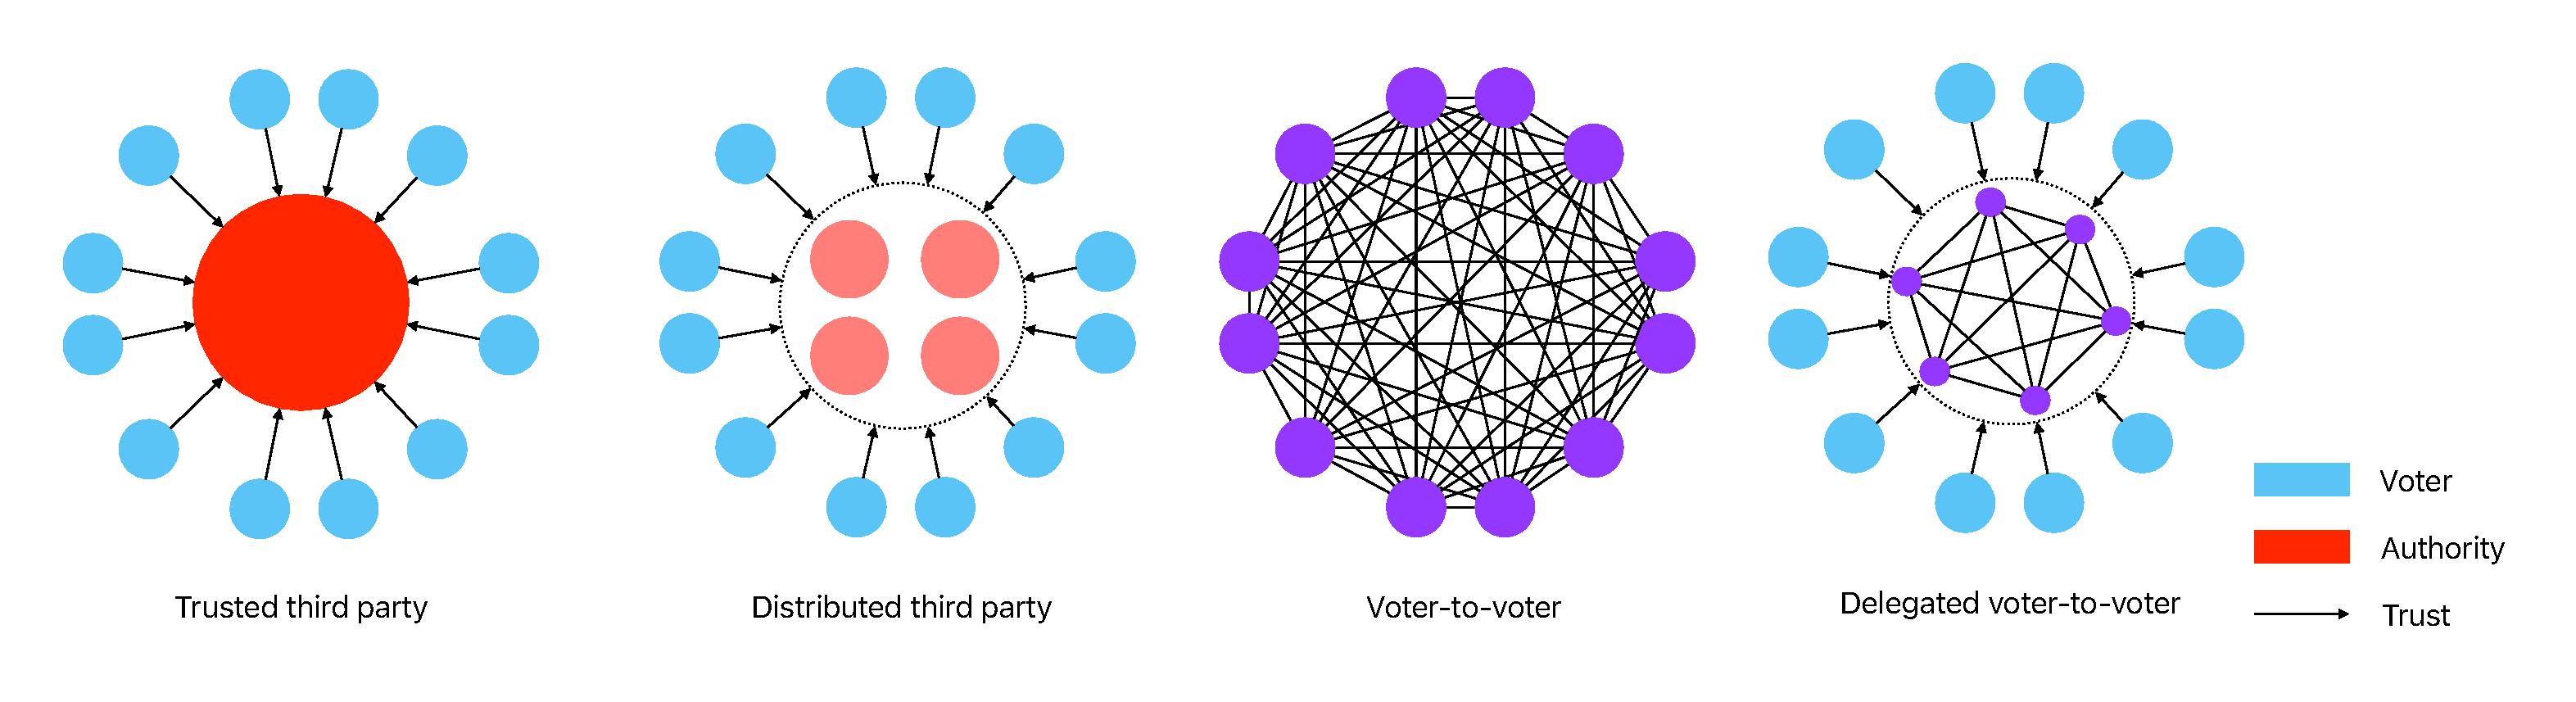
\includegraphics[width=\textwidth]{trust-models-voting.pdf}
    \caption{Four trust models: trusted third party, distributed third part, voter-to-voter, and delegated voter-to-voter}
    \label{fig:trust-models}
\end{figure*}

Protocols using a distributed set of authorities typically use Distributed Key Generation (DKG) \cite{gennaroSecureDistributedKey1999} to jointly generate encryption keys. The integrity of the voting process is maintained under the assumption of an 'honest majority', where privacy is preserved provided there is no collusion between the parties. However, the traditional DKG model faces challenges in voting systems, particularly when parties involved in the DKG are unavailable, potentially disrupting the voting process \cite{haoAnonymousVotingTworound2010}. While this may not be an issue for government-level elections, in smaller elections collateral deposits may be required to incentivise participation \cite{elsheikhDisputefreeScalableOpen2022}, we find this approach impractical for wider applications. Instead, we propose a protocol based on threshold cryptography that tolerates a certain level of node unavailability. Our contributions are as follows:

\begin{enumerate}
    \item We present an Internet voting protocol based on a delegated voter-to-voter trust model. This model reflects the trust relationships within a group and expresses them in the security and availability properties of the system. It is particularly suitable for small-scale elections where participants are familiar with each other and existing trust lines are established.
    
    \item We develop a new technique for dynamic Distributed Key Generation (DKG), called Federated DKG (FDKG). FDKG facilitates joint key pair generation by members with a single message exchange, without prior knowledge of all participants.

    \item We propose a solution to the problem of node unavailability, which can hinder the election process. Using threshold cryptography and the concept of Guardian Sets, each participant shares its secret with a selected set of trusted nodes. Provided that these Guardian Sets consist of reputable and reliable network members, the risk of failure or collusion is minimised. This ensures that the improved availability of our protocol does not compromise its security.
    
    \item We outline a practical implementation strategy for a peer-to-peer environment with no transaction fees, and an alternative public blockchain implementation using a single paymaster. This approach offers a significant advantage over existing protocols that require hosting or per-vote fees.

    \item We present an open source implementation of our protocol in TypeScript and Golang, improving its cross-platform adaptability and thereby increasing its accessibility and practical utility.
\end{enumerate}

\section{Related Work}
Internet voting protocols typically rely on a trusted third party, with variations in server capabilities determining integrity, anonymity, privacy, censorship resistance, and coercion resistance based on the trustworthiness of that entity. Current research mainly uses blockchain technology for its integrity and transparency in vote storage, as seen in systems such as Voatz, Polys, Follow My Vote, Verify-Your-Vote, OpenVoteNetwork, TIVI, Stellot, Votem, Cicada, Aragon/Vocdoni and MACI~\cite{mooreWestVirginiaMobile2019, PolysOnlineVoting, SecureDecentralizedApplication2023, chaiebVerifyYourVoteVerifiableBlockchainBased2019, haoAnonymousVotingTworound2010, mccorrySmartContractBoardroom2017, seifelnasrScalableOpenVoteNetwork2020, elsheikhDisputefreeScalableOpen2022, TIVIPoweredSmartmatic, NowYouCan2016, baranskiPracticalIVotingStellar2020, votemcorpVotemProofofvoteVotem, BuildingCicadaPrivate, A16zCicada2023, ethereumfoundationMinimalAntiCollusionInfrastructure2022, VocdoniIntroductionVocdoni, PrivacyscalingexplorationsMaci2023}.

Alternatively, projects such as Helios, Civitas, Swisspost/Scytl, CHVote, iVoting and ElectionGuard use distributed authority and multi-party computation (MPC) protocols without explicitly relying on blockchain technology \cite{adidaHeliosWebbasedOpenAudit2008, clarksonCivitasSecureVoting2008, 
CHVoteProjectRelease,roenneJCJImprovedVerifiability2016, benalohElectionGuardDesignSpecification2023}. These systems are not fully decentralised, relying on a closed set of trusted entities known as Guardians.

Public blockchain-based solutions typically struggle with usability and require voters to pay transaction fees. Non-blockchain solutions operate either in a SaaS model or as self-hosting software, shifting the operational burden to election organisers and potentially creating accessibility barriers for small-scale voting and non-technical operators. Hybrid systems, like MACI, require both a blockchain network and a single coordinator server \cite{ethereumfoundationMinimalAntiCollusionInfrastructure2022, PrivacyscalingexplorationsMaci2023}.

Our proposed solution differs significantly from these models. It is free, unlike public blockchain-based systems, potentially increasing voter participation. Unlike private blockchain-based systems, our protocol operates without centralised servers, making it particularly suitable for smaller, informal voting settings. This approach shifts the trust paradigm from central authorities to the voters themselves.


\newcommand{\fullmoon}{\tikz\filldraw[fill=black] (0,0) circle (0.5em);}
\newcommand{\newmoon}{\tikz\draw (0,0) circle (0.5em);}
\newcommand{\rightmoon}{\tikz\draw (0,0) circle (0.5em); \filldraw[fill=black] (0,0) arc (90:270:0.5em) -- cycle;}
\newcommand{\leftmoon}{\tikz\draw (0,0) circle (0.5em); \filldraw[fill=black] (0,0) arc (270:90:0.5em) -- cycle;}
\newcommand{\halfmoon}{\tikz\draw (0,0) circle (0.5em); \filldraw[fill=black] (0,-0.5em) rectangle (0,0.5em);}


\begin{table*}[!h]
\centering
\newcommand{\YES}{\cellcolor{red!50}Yes}
\newcommand{\NO}{\cellcolor{green!50}No}
\begin{tabular}{p{0.2\textwidth}p{0.2\textwidth}p{0.17\textwidth}p{0.17\textwidth}p{0.21\textwidth}}
\noalign{\smallskip}\hline\noalign{\smallskip}
\textbf{Property} & \textbf{Central server} & \textbf{Private network} & \textbf{Public blockchain} & \textbf{Voter-to-voter network}\\
\noalign{\smallskip}\hline\noalign{\smallskip}
Transaction fees & \NO & \NO & \YES & \NO \\
\hline
Service cost & \cellcolor{yellow!50} Medium & \cellcolor{red!50} High & \cellcolor{green!50} No  & \cellcolor{green!50} No \\
\hline
Ease of use & \cellcolor{green!50} High & \cellcolor{green!50}High & \cellcolor{red!50} Low & \cellcolor{yellow!50} Medium \\
\hline
Trust to & \cellcolor{red!50} Central authority & \cellcolor{yellow!50} Authorities & \cellcolor{yellow!50} Miners & \cellcolor{yellow!50} Voters  \\
\noalign{\smallskip}\hline
\hline
\end{tabular}

\caption{A comparative analysis of four types of Internet voting protocols: central server, private network, public blockchain, and voter-to-voter network, highlighting their differences in transaction fees, service costs, ease of use, and trust dynamics, where trust refers to an entity that guarantees properties of censorship resistance, privacy, and correctness. Examples of authorities are: "Returning Officers, members of the Board of Trustees, government officials or other trusted authorities who are responsible and accountable for the conduct of the election"~\cite{benalohElectionGuardDesignSpecification2023}. The service cost includes all costs related to running the software like implementation, maintenance, and fees.}
\label{table-comparision}

\end{table*}

Furthermore, various systems achieve different security and privacy properties depending on their underlying assumptions. For example, OpenVoteNetwork eliminates the need for trusted third parties by adopting a self-tallying scheme, which ensures perfect ballot secrecy but is vulnerable to denial of service attacks \cite{haoAnonymousVotingTworound2010, mccorrySmartContractBoardroom2017, seifelnasrScalableOpenVoteNetwork2020, elsheikhDisputefreeScalableOpen2022}.

Minimal Anti-collusion Infrastructure (MACI), guarantees the highest level of security, i.e., censorship resistance, privacy, voter anonymity, and coercion resistance, however, the ballot privacy relies on a single coordinator server~\cite{ethereumfoundationMinimalAntiCollusionInfrastructure2022, PrivacyscalingexplorationsMaci2023}.

Cicida achieves ballot secrecy using homomorphic time-lock puzzles and voter anonimity using Semaphore for zero-knowledge set membership proofs \cite{BuildingCicadaPrivate, A16zCicada2023}.

Aragon/Vocdoni, like Cicida, achieves voter anonymity using zero-knowledge set membership proofs, but election secrecy is achieved using trusted nodes called KeyKeepers. When a new election is created, each KeyKeeper creates an encryption key and publishes the public part via a transaction (setProcessKeysTx). The voters select up to N (at least one) of the keys and encrypt the vote with the N keys in onion mode~\cite{williamsRemoteVotingAge2022, VocdoniIntroductionVocdoni}. 

Votem~\cite{votemcorpVotemProofofvoteVotem}, achieves voter anonymity using a re-encryption mix network. Election secrecy is achieved using ElGamal homomorphic encryption and Distributed Key Generation (DKG) and Multi-Party Computation (MPC) for decryption. Votem uses permissioned blockchain network, where each node is explicitly granted a set of permissions by the authority conducting the election.

ElectionGuard~\cite{benalohElectionGuardDesignSpecification2023} uses a similar approach to DKG/MPC with threshold homomorphic encryption, without explicitly relying on blockchain technology or consensus algorithms. Instead, it uses a set of permissioned nodes called Guardians.

Our protocol follows the same approach of DKG/MPC/ElGamal/threshold encryption, but generalises the trust model by allowing each voter to act as a Guardian and share their secret input with a set of trusted parties. This model not only further decentralises trust, but also enhances privacy and security by distributing the power of vote verification among a wider set of participants. 


\paragraph{Objectives}
In designing the protocol, we focused on key objectives to address the essential challenges and needs of a secure and practical Internet voting protocol. These objectives are

\begin{enumerate}
    \item \textbf{Distributed Model.} Use a fully distributed model to eliminate the need for central authorities or trusted intermediaries. This approach increases the resilience of the system to attack and reduces the risk of single points of failure.
    \item \textbf{Flexible Trust.} Use a social mapping approach to security, where the system relies on the structure of trust within the community. People who are more trusted should have a greater role in maintaining security.
    \item \textbf{Privacy.} Ensure voter anonymity and vote secrecy using cryptographic methods based on the honest-trust-majority assumption. This means that individual votes remain secret and cannot be decrypted unless the most important nodes collude.
    \item \textbf{Robustness}: The protocol should be robust to partial participation, especially in the final round, allowing for flexible participation without compromising the integrity of the voting process.
    \item \textbf{Accessibility}. Ensure that the protocol works smoothly on common devices such as smartphones and laptops. This makes it accessible, scalable and easy to use for everyone.
\end{enumerate}


% Party
\newcommand{\PartySecretKey}[1]{\ensuremath{s_{#1}}}
\newcommand{\Party}[1]{\ensuremath{P_{#1}}}
\newcommand{\Parties}{\ensuremath{\mathbb{P}}}
\newcommand{\VotesSize}{\ensuremath{|\mathbb{V}}|}

% Voting keys
\newcommand{\EncryptionKey}{\textbf{E}}
\newcommand{\DecryptionKey}{\textbf{d}}

% Partial voting keys
\newcommand{\PartialDecryptionKey}[1]{\ensuremath{d_{#1}}}
\newcommand{\PartialEncryptionKey}[1]{\ensuremath{E_{#1}}}

% Ciphertexts
\newcommand{\EncryptedPartialDecryptionKeyShare}[2]{\ensuremath{C_{#1,#2}}}
\newcommand{\SetOfEncryptedPartialDecryptionKeys}{\ensuremath{\mathbb{C}}}
\newcommand{\SetOfFDKG}{\ensuremath{\mathbb{D}}}
\newcommand{\SetOfSharesOfPartialDecryption}{\ensuremath{\mathbb{C}}}
\newcommand{\Voters}{\ensuremath{\mathbb{V}}}
\newcommand{\Tallies}{\ensuremath{\mathbb{T}}}
% Shares
\newcommand{\IthDecryptionKey}[1]{\ensuremath{d_{#1}}}
\newcommand{\IthEncryptionKey}[1]{E_{#1}}

% Private channel
\newcommand{\DecryptionUsingOf}[2]{\ensuremath{\texttt{Dec}_{#1}(#2)}}
\newcommand{\EncryptionUsingOf}[2]{\ensuremath{\texttt{Enc}_{#1}(#2)}}

\newcommand{\PartialDecryptionKeyShare}[2]{\ensuremath{[d_{#1}]_{#2}}}


\newcommand{\ProofFDKG}[1]{\ensuremath{\textrm{PROOF}_{\textrm{FDKG}_{#1}}}}

\newcommand{\ProofFDKGInformal}{"Given \PartialEncryptionKey{i}, \EncryptedPartialDecryptionKeyShare{i}{j} and $\Party{j} \in \GuardianSetOf{i}$, I know $f_i = a_0, \dots, a_{t-1}$, $r1_1,\dots,r1_k$, and $r2_1,\dots,r2_k$, s.t. $\PartialEncryptionKey{i}=a_0G$ and the \EncryptedPartialDecryptionKeyShare{i}{j} is an encrypted value of a polynomial $f_i$ applied to $j$"}

\newcommand{\ProofBALLOT}[1]{\ensuremath{\textrm{PROOF}_{\textrm{\Ballot{#1}}}}}

\newcommand{\ProofBALLOTInformal}{"Given \EncryptionKey{} and \Ballot{i} = $(C1, C2)$, I know \BlindingFactor{i}, and \Vote{i} s.t. $\Vote{i} \in \{2^0, 2^j, \ldots, 2^{(l-1)j}\}$ and $\Ballot{i} = (\BlindingFactor{i} G,\ \BlindingFactor{i} \EncryptionKey{} + \Vote{i})$"}

\newcommand{\ProofPD}[1]{\ensuremath{\textrm{PROOF}_{\PartialDecryptionFrom{#1}}}}

\newcommand{\ProofPDInformal}{"Given $\TotalA{}, \PartialDecryptionFrom{i}, \PartialEncryptionKey{i}$, I know a partial decryption key $\PartialDecryptionKey{i}$ s.t. $\PartialEncryptionKey{i} = \PartialDecryptionKey{i} G$ and $\PartialDecryptionFrom{i} = \PartialDecryptionKey{i} \TotalA{}$"}

\newcommand{\ProofPDS}[2]{\ensuremath{\textrm{PROOF}_{\SharePartialDecryptionFromTo{#1}{#2}}}}

\newcommand{\ProofPDSInformal}{"Given $\SharePartialDecryptionFromTo{j}{i}, \EncryptedPartialDecryptionKeyShare{j}{i}, \TotalA$, I know a secret key $\PartySecretKey{i}$ s.t. $\SharePartialDecryptionFromTo{j}{i} = \TotalA  \PartialDecryptionKeyShare{j}{i}$ where $\PartialDecryptionKeyShare{j}{i} = \DecryptionUsingOf{\PartySecretKey{i}}{\EncryptedPartialDecryptionKeyShare{j}{i}}$"}



\newcommand{\Ballot}[1]{\ensuremath{B_{#1}}}

\newcommand{\Generator}[1]{\ensuremath{H_{#1}}}
\newcommand{\BlindingFactor}[1]{\ensuremath{r_{i}}}
\newcommand{\Vote}[1]{\ensuremath{v_{#1}}}

\newcommand{\GuardianSetOf}[1]{\ensuremath{\mathbb{G}_{#1}}}
\newcommand{\TotalA}{\ensuremath{C1}}
\newcommand{\TotalB}{\ensuremath{C2}}
\newcommand{\BallotA}[1]{\ensuremath{C1_{#1}}}
\newcommand{\BallotB}[1]{\ensuremath{C2_{#1}}}

\newcommand{\G}{\ensuremath{G}}


% Partial Decryption Results
\newcommand{\SharePartialDecryptionFromTo}[2]{\ensuremath{[\mathrm{PD}_{#1}]_{#2}}}

\newcommand{\PartialDecryptionFrom}[1]{\ensuremath{\mathrm{PD}_{#1}}}

\section{Preliminaries}
In this section, we outline essential cryptographic concepts and tools that underlie the PeerVote protocol presented in this paper. These preliminaries provide the necessary background for understanding the structure and functionality of our protocol.


% Table of Notations
\begin{table}[h]

\caption{Summary of Notations}
\label{tab:notations}
\begin{tabular}{>{\centering\arraybackslash}p{.2\linewidth}p{.8\linewidth}}

\hline
\textbf{Notation} & \multicolumn{1}{c}{\textbf{Description}} \\
\hline

\Parties          & Set of all parties $\Party{i} \in \Parties$ in the voting process \\

\Party{i},\PartySecretKey{i} & Public and secret keys used to authenticate $i$-th party, where $\Party{i}=\PartySecretKey{i} \G$  \\

\hline

$\SetOfFDKG \subseteq \Parties$ & Subset of parties involved in the 1. FDKG phase  \\

\PartialEncryptionKey{i},\PartialDecryptionKey{i}      & Partial encryption (public) and decryption (secret) keys of \Party{i}. $\PartialEncryptionKey{i}=\PartialDecryptionKey{i} \G$, where $\PartialDecryptionKey{i}$ is a random ephemeral (per vote) scalar value.  \\

\EncryptionKey{}, \DecryptionKey{}    & Voting public (encryption) and secret (decryption) keys, that is a sum of partial encryption keys \PartialEncryptionKey{i}, and decryption keys \PartialDecryptionKey{i} accordingly \\

$\GuardianSetOf{i}$ & Guardian set is a subset of parties  selected by \Party{i} that can recreate \Party{i}'s part of the decryption key \PartialDecryptionKey{i}.  $\GuardianSetOf{i} \subseteq \Parties \setminus \Party{i}$ \\

$k = |\GuardianSetOf{}|$                 & Total number of parties in a guardian set \\

$t$                 & Threshold number to reconstruct the shared secret \\

\PartialDecryptionKeyShare{i}{j}      & Share of partial decryption (secret) key, from \Party{i} to \Party{j}   \\

\hline

$\Voters \subseteq \Parties$ & Subset of parties participating in the 2. Voting phase  \\

$v_i$             & Encoded vote of \Party{i} \\

$\BlindingFactor{i}$ & One-time random value used for secure ElGamal encryption \\

$\Ballot{i}=(\BallotA{i}, \BallotB{i})$     & Encrypted ballot of participant \Party{i} using ElGamal scheme consisting of $(\BallotA{i}, \BallotB{i})$, where $\BallotA{i}=\BlindingFactor{i} \G$, and $\BallotB{i} = \BlindingFactor{i} \EncryptionKey{} + \Vote{i} \G$ \\

\hline

$\Tallies \subseteq \Parties$ & Subset of parties  participating in the 3. Online Tally phase \\

\TotalA     & Sum of the first parts of all the casted ballots, i.e., $\TotalA = \sum_{\Party{i} \in \Voters} \BallotA{i}$ \\

\TotalB     & Sum of the second parts of all the casted ballots, i.e., $\TotalB = \sum_{\Party{i} \in \Voters} \BallotB{i}$ \\


\PartialDecryptionFrom{i}      & Partial decryption from \Party{i}, i.e., $\PartialDecryptionFrom{i} = \PartialDecryptionKey{i} \TotalA$ \\

\SharePartialDecryptionFromTo{i}{j} & Share of partial decryption, from \Party{i} to \Party{j}, i.e., $\SharePartialDecryptionFromTo{i}{j} = \PartialDecryptionKeyShare{i}{j} \TotalA$ \\

\hline

$\texttt{Enc}_{\Party{i}}, \texttt{Dec}_{\PartySecretKey{i}}$ & Public key encryption for \Party{i} and decryption using the corresponding secret key $\PartySecretKey{i}$, as described in Appendix~\ref{private-channel} \\

$\Delta$ & A helper value used to encode a scalar value to a point on a curve \\

\EncryptedPartialDecryptionKeyShare{i}{j} & Encrypted partial decryption key share, from \Party{i} to \Party{j}  \\

\hline

\ProofBALLOT{i} & zkSNARK proof of correctness of \Ballot{i}\\

\ProofFDKG{i} & zkSNARK proof of correctness of (\PartialDecryptionKey{i}, \EncryptedPartialDecryptionKeyShare{i}{}) \\

\ProofPD{i} & zkSNARK proof of correctness of  \PartialDecryptionFrom{i} \\

\ProofPDS{i}{j} & zkSNARK proof of correctness of \SharePartialDecryptionFromTo{i}{j}  \\
\end{tabular}
\end{table}


\subsection{zk-SNARK}

zk-SNARKs are cryptographic tools that allow one party (the prover) to prove to another (the verifier) the truth of a statement without revealing any information beyond the validity of the statement \cite{grothSizePairingbasedNoninteractive2016}.

Consider an arithmetic circuit $C$ characterised by a relation $\mathcal{R}_C$ and a language $\mathcal{L}_C$. This circuit accepts a statement $\vec{s}$ and a witness $\vec{w}$ such that $(\vec{s}, \vec{w}) \in \mathcal{R}_C$. A zk-SNARK for the satisfiability of this circuit is defined by three polynomial-time algorithms ~\cite{grothSizePairingbasedNoninteractive2016,parnoPinocchioNearlyPractical2013}:
\begin{itemize}
    \item $\textrm{(pk,vk)} \gets \textrm{Setup}(1^\lambda,C)$. For a given security parameter $\lambda$ and the circuit $C$, this algorithm produces a common reference string (CRS) comprising a proving key $\textrm{pk}$ and a verifying key $\textrm{vk}$, both of which are public parameters associated with the circuit $C$.
    \item $\pi \gets \textrm{Prove}(\textrm{pk}, \vec{s}, \vec{w})$. Using the proving key $\textrm{pk}$, the statement $\vec{s}$, and the witness $\vec{w}$ such that $(\vec{s}, \vec{w}) \in \mathcal{R}_C$, this algorithm generates a non-interactive zero-knowledge proof $\pi$ for the statement $\vec{s} \in \mathcal{L}_C$, demonstrating the relationship between $\vec{s}$ and $\vec{w}$.
    \item $0/1 \gets \textrm{Verify}(\textrm{vk}, \vec{s}, \pi)$. With the verifying key $\textrm{vk}$, the statement $\vec{s}$, and the proof $\pi$, this algorithm outputs 1 if $\pi$ is a valid proof for the statement $\vec{s} \in \mathcal{L}_C$, and outputs 0 otherwise.
\end{itemize}


\subsection{Federated Distributed Key Generation}
The Distributed Key Generation (DKG) protocol aims to collectively generate a voting encryption key pair without any single participant learning the secret (decryption) key. Each party $P_i \in \mathbb{P}$ learns only its share of this key, while the public (encryption) key is widely known. The protocol uses threshold cryptography, which allows flexibility in the participation of the participants during the tallying phase.

\subsubsection*{Secret Sharing}
Secret sharing via Shamir's Secret Sharing (SSS) scheme enables a dealer to distribute a secret key $s$ over a randomly chosen polynomial $\mathbf{f}(X) = a_0 + a_1X + a_2X^2 + \dots + a_{t-1}X^{t-1}$, where coefficients $a_0,a_1,\dots,a_{t-1} \in_R \mathbb{F}_q$. Here, the secret key $s=a_0=\mathbf{f}(0)$ and $t-1$ denotes the polynomial's degree. Shares are computed by evaluating $\mathbf{f}(i)$ for $i \neq 0$. Using Lagrange's Theorem, reconstructing $\mathbf{f}(X)$ and hence extracting $s = \mathbf{f}(0)$ is possible with $t$ points on the polynomial.

\subsubsection*{Distributed Key Generation}
To avoid centralising the role of the dealer (and revealing the secret value $s$), the generation of polynomial $\mathbf{f}(X) \in_R \mathbb{Z}_q[X]$ is distributed among all parties $\mathbb{P}$. Each party selects a random polynomial $f_{i}(X) \in \mathbb{Z}_q[X]$, and the final polynomial is the sum of these individual polynomials: \[\mathbf{f}(X)=\sum_{i=1}^{n}f_i(X)\] Consequently, the voting secret (decryption) key $\mathbf{d}$ and voting public (encryption) key $\mathbf{E}$ are defined as: $$\mathbf{d}=\mathbf{f}(0)$$ $$\mathbf{E}=\mathbf{d} \G$$ 
To prevent arbitrary submissions by parties, Publicly Verifiable Secret Sharing (PVSS) is used, incorporating zero-knowledge proofs to validate the correctness of shared values \cite{goosSimplePubliclyVerifiable1999}.

\subsubsection*{Dynamic Distributed Key Generation}
Traditional DKG requires a known, fixed number of participants due to its reliance on SSS with predefined polynomial degrees. As we are aiming for an optional DKG phase with an unpredictable number of participants, we need a mechanism that allows dynamic adjustments to the number of participants.

Existing dynamic DKG schemes, such as the one in \cite{delerableeDynamicThresholdPublickey2008}, necessitate continuous online presence of all parties, which we find impractical. Our objective is a non-interactive protocol where parties send only a single message and are then free to leave (You Only Speak Once approach~\cite{gentryYOSOYouOnly2021}). We propose Federated DKG which facilitates joint key establishment by members with a single message, without prior knowledge of all participants.
The technique works similar to the Federated Byzantine Agreement (FBA) used in the Stellar Consensus Protocol \cite{mazieresStellarConsensusProtocol2015}. The details are described in the next section.

\section{Voting Protocol}

Our protocol integrates the three-round voting scheme from \cite{schoenmakersLectureNotesCryptographic2018}, the multi-candidate encoding method from \cite{haoAnonymousVotingTworound2010}, and the Federated Distributed Key Generation (FDKG) introduced in this paper.

\paragraph*{Assumptions}
The protocol is based on the following assumptions:
\begin{enumerate}
\item All communications occur over a public message board available to all parties.
\item Parties are identified only by their public keys \Party{i} and authenticated by their secret keys \PartySecretKey{i}.
\item Private channels over public message board are secured using encryption functions $\texttt{Enc}_{\Party{i}}$ and $\texttt{Dec}_{\PartySecretKey{i}}$ described in Appendix~\ref{private-channel}.
\item Each party verifies zkSNARK proofs and rejects messages that fail verification.
\item Participants consent to certain cryptographic parameters, including the BabyJubJub Elliptic Curve~\cite{whitehatBabyJubjubElliptic2020} $E(\mathbb{Z}_p)$ with a defined curve finite field modulus $p$, a base point $G$ on the curve, and the order of the base point $q$. Additionally, they agree to the set of eligible voters $\mathbb{P}$ and the set of candidates.
\end{enumerate}

\subsection{Round 1: Federated Distributed Key Generation}
Participation in the FDKG phase is optional. For each participating party $\Party{i} \in \mathbb{D}$, where $\mathbb{D} \subseteq  \mathbb{P}$:
\begin{enumerate}
    \item A guardian set of $k$ parties $\mathbb{G}_i\subseteq \mathbb{P}/P_i$ is selected based on the established trust lines of \Party{i}.
    \item A random polynomial $f_{i}(X) \in_{\$} \mathbb{Z}_q[X]$ of degree $t-1$ is sampled.
    \item Partial decryption (secret) key $\PartialDecryptionKey{i}= f_i(0)$ and partial encryption (public) key $\PartialEncryptionKey{i} = \PartialDecryptionKey{i} \G$ are computed.
    \item A t-of-k access structure for \PartialDecryptionKey{i} is created using PVSS. For each guardian $P_{j} \in \mathbb{G}_i$, partial decryption key share $\PartialDecryptionKeyShare{i}{j}=f_i(j)$ is encrypted as $\EncryptedPartialDecryptionKeyShare{i}{j}=\EncryptionUsingOf{\Party{j}}{\PartialDecryptionKeyShare{i}{j}}$ as described in Appendix~\ref{private-channel}.
    % \item A zero-knowledge proof \ProofFDKG{i} is created (see Section~\ref{sec:proof-fdkg}) and broadcast along with (\PartialEncryptionKey{i}, \EncryptedPartialDecryptionKeyShare{i}{j}).
    
    \item Compute a zero-knowledge proof \ProofFDKG{i}, as described in Section~\ref{sec:proof-fdkg}.
    
    \item Broadcast (\PartialEncryptionKey{i}, \EncryptedPartialDecryptionKeyShare{i}{j}, \ProofFDKG{i}).
\end{enumerate}

\paragraph*{State after Round 1:}
Upon completion of FDKG, the message board contains:
\begin{itemize}
    \item $\{\PartialEncryptionKey{i} : \Party{i} \in \mathbb{D}\}$, the set of partial encryption keys, where \EncryptionKey{} can be reconstructed by anyone by summing $\EncryptionKey=\sum_{\Party{i} \in \mathbb{D}} \PartialEncryptionKey{i}$.
    \item $\bigcup_{\Party{i} \in \mathbb{D}} \{C_{i,j} \mid P_j \in \mathbb{G}_i\}$, the set of encrypted shares of the partial decryption keys.  
\end{itemize}

\newpage
\subsection{Round 2: Casting Votes}

For each voter $\Party{i} \in \mathbb{V}$, where $\mathbb{V} \subseteq  \mathbb{P}$:

\begin{enumerate}
    \item Encode a multi-candidate ballot using the method outlined in \cite{baudronPracticalMulticandidateElection2001}. The encoding assigns a power of two to each candidate: a vote for candidate 1 as $2^0$, for candidate 2 as $2^m$, for candidate $c$ as $2^{(c-1)m}$. The parameter $m$ is selected as the smallest integer where $2^m > |\Parties{}|$. Thus, a vote is defined as \[\Vote{i}\ =\ \begin{cases} 2^0 & \text{if } \Party{i} \text{ votes for candidate 1} \\ 2^m & \text{if } \Party{i} \text{ votes for candidate 2} \\ \vdots & \vdots \\ 2^{(c-1)m} & \text{if } \Party{i} \text{ votes for candidate $c$}\end{cases}\]
    
    \item Encrypt the vote using ElGamal encryption as $\Ballot{i} = (\BlindingFactor{i} \G,\ \BlindingFactor{i} \EncryptionKey{} + \Vote{i} \G)$, where $\BlindingFactor{i} \in_{\$} \mathbb{Z}_q$ serves as a one-time blinding value.
    
    \item Compute a zero-knowledge proof \ProofBALLOT{i}, as described in Section~\ref{sec:proof-ballot}.
    
    \item Broadcast $(\Ballot{i}, \ProofBALLOT{i})$.
\end{enumerate}

\paragraph{State after Voting}

Once the voting phase concludes (either when $|\Parties|$ messages have been received or after a predefined period), the message board's state is appended with:
\begin{itemize}
    \item $\{\Ballot{i} : \Party{i} \in \Voters\}$, the set of encrypted votes.
\end{itemize}



\subsection{Round 3: Tally}

The tally process consists of two distinct phases: online and offline.

\subsubsection{Online Tally}

The subset of parties $\Tallies \subseteq \Parties$ involved in Threshold ElGamal decryption includes at least $t$ parties from each guardian set \GuardianSetOf{1},\dots,\GuardianSetOf{|\SetOfFDKG|}. For each party $\Party{i} \in \mathbb{T}$:


\begin{enumerate}
    \item Sum the first component of all ballots $\TotalA = \sum_{\Party{i} \in \mathbb{V}} \BallotA{i}$, where (\BallotA{i},\BallotB{i})=\Ballot{i}.

    \item If $\Party{i} \in \SetOfFDKG$:
        \begin{enumerate}
            \item Compute the partial decryption $\PartialDecryptionFrom{i} = \PartialDecryptionKey{i} \TotalA$.
            \item Generate a zero-knowledge proof \ProofPD{i} (as described in Section~\ref{sec:proof-pd}).
            \item Broadcast $(\PartialDecryptionFrom{i},\ProofPD{i})$.
        \end{enumerate}
    
    \item For each received encrypted share $\EncryptedPartialDecryptionKeyShare{j}{i}$, where $\Party{j} \in \mathbb{D} \setminus \{\Party{i}\}$ and $\Party{i} \in \GuardianSetOf{j}$:
        \begin{enumerate}
            \item Decrypt to obtain \PartialDecryptionKeyShare{j}{i}=\DecryptionUsingOf{\PartySecretKey{i}}{\EncryptedPartialDecryptionKeyShare{j}{i}}.
            \item Calculate the share of partial decryption $\SharePartialDecryptionFromTo{j}{i} = \PartialDecryptionKeyShare{j}{i} \TotalA$.
            \item Generate a zero-knowledge proof \ProofPDS{j}{i} (outlined in Section~\ref{sec:proof-pds}).
            \item Broadcast $(\SharePartialDecryptionFromTo{j}{i},\ProofPDS{j}{i})$.
        \end{enumerate}
\end{enumerate}

\paragraph{State after Online Tally}

After completing the Online Tally (the set is decryptable as defined in Definition~\ref{def:decipherability}), the message board's state is appended with:
\begin{itemize}
    \item $\{\PartialDecryptionFrom{i} :  \Party{i} \in \mathbb{D} \land \Party{i} \in \mathbb{T}\}$, the set of partial decryptions.
    
    \item $\bigcup_{\Party{i} \in \mathbb{T}} \{\SharePartialDecryptionFromTo{j}{i} : \Party{j} \in \mathbb{D} \setminus \{\Party{i}\} \text{ and } \Party{i} \in \GuardianSetOf{j}\}$, the set of shares of partial decryption.
\end{itemize}

\subsubsection{Offline Tally}

The Offline Tally phase is accessible to anyone and involves the following steps:

\begin{enumerate}
    \item Sum the second component of all ballots $\TotalB = \sum_{\Party{i} \in \Voters} \BallotB{i}$, where (\BallotA{i},\BallotB{i})=\Ballot{i}.
    
    \item Calculate the sum of either partial decryptions or their reconstructions from shares: \[Z = \sum\{\PartialDecryptionFrom{i} \textrm{ or } \sum (\SharePartialDecryptionFromTo{i}{j} \lambda_{j}) : \Party{j} \in \GuardianSetOf{i}\} = \DecryptionKey{} \TotalA = \mathbf{d} \sum_{\Party{i} \in \Voters} r_i G \] where $\lambda_{i}=\Pi_{j \neq i}\frac{j}{j-i}$ represents the Lagrange coefficient.

    \item The decryption is $M=\TotalB{} - Z=(x_1 2^0 + x_2 2^j + \dots + x_l 2^{(l-1)j}) \G$, where $x_i$ is the number of votes for candidate $i$. It is because 
    
    $\begin{aligned} M&=\TotalB-Z \\
        &= (\sum_{\Party{i} \in \Voters} r_{i} \mathbf{E} + \sum^{x_1} 2^0 \G + \sum^{x_2} 2^j \G + \dots + \sum^{x_l} 2^{(l-1)j} \G ) - Z \\
        &= \sum_{\Party{i} \in \Voters} r_{i} \mathbf{E} + (x_1 2^0 + x_2 2^j + \dots + x_l 2^{(l-1)j}) \G - \mathbf{d} \sum_{\Party{i} \in \Voters} r_i \G \\
        &= \sum_{\Party{i} \in \Voters} r_{i} \mathbf{E} + (x_1 2^0 + x_2 2^j + \dots + x_l 2^{(l-1)j})\G - \sum_{\Party{i} \in \Voters} r_{i} \mathbf{E}\\
        &= (x_1 2^0 + x_2 2^j + \dots + x_l 2^{(l-1)j}) \G\\
        \end{aligned}$
    
    \item Extract each $x_i$ by solving the Discrete Logarithm Problem. Given the small range of $x_i$ ($0 \leq x_i \leq |\mathbb{V}|$), this is a feasible task. The extraction technique for each $x_i$ follows the method described in \cite{haoAnonymousVotingTworound2010}.
\end{enumerate}





\subsection{Proofs Constructions}\label{sec:proofs}

In our protocol, we employ the general principles of zk-SNARK to construct specific proofs for each phase of the voting process. Each proof is defined by a circuit $C$ that verifies constraints, a public instance (statement) $\vec{s}$, and a private input (witness) $\vec{w}$.

\subsubsection{\ProofFDKG{i}}\label{sec:proof-fdkg}

\begin{itemize}
    \item \textbf{Circuit} ($C$): Defined as \ProofFDKGInformal{}. The specifics of this circuit are detailed in Algorithm~\ref{alg:circuit_fdkg}.
    \item \textbf{Public Instance} ($\vec{s}$): Includes the partial encryption key $\PartialEncryptionKey{i}$, the guardian set $\GuardianSetOf{i} = \{\Party{1},\dots,\Party{|\GuardianSetOf{}|}\}$, and the set of encrypted partial decryption key shares $\{\EncryptedPartialDecryptionKeyShare{}{1},\dots, \EncryptedPartialDecryptionKeyShare{}{|\GuardianSetOf{}|}\}$.
    \item \textbf{Private Input} ($\vec{w}$): Includes the coefficients of the polynomial $\{a_0, \dots, a_{t-1}\}$ and random values $\{r1_1,\dots,r1_{|\GuardianSetOf{}|}\}$, $\{r2_1,\dots,r2_{|\GuardianSetOf{}|}\}$.
\end{itemize}

\subsubsection{\ProofBALLOT{i}}\label{sec:proof-ballot}

\begin{itemize}
    \item \textbf{Circuit} ($C$): Defined as \ProofBALLOTInformal{}. Algorithm~\ref{alg:circuit_proof_ballot} elaborates on this circuit.
    \item \textbf{Public Instance} ($\vec{s}$): Includes the encryption key $\EncryptionKey{}$ and the encrypted ballot $\Ballot{i} = (C1, C2)$.
    \item \textbf{Private Input} ($\vec{w}$): Includes the vote $\Vote{i}$ and the random blinding factor $r_i$.
\end{itemize}

\subsubsection{\ProofPD{i}}\label{sec:proof-pd}

\begin{itemize}
    \item \textbf{Circuit} ($C$): Specified as \ProofPDInformal{}. Details of this circuit can be found in Algorithm~\ref{alg:circuit_proof_pd}.
    \item \textbf{Public Instance} ($\vec{s}$): Includes the sum of first ballot components $\TotalA{}$, the partial decryption from party $\PartialDecryptionFrom{i}$, and the partial encryption key $\PartialEncryptionKey{i}$.
    \item \textbf{Private Input} ($\vec{w}$): Includes the partial decryption key $\PartialDecryptionKey{i}$.
\end{itemize}

\subsubsection{\ProofPDS{i}{j}}\label{sec:proof-pds}

\begin{itemize}
    \item \textbf{Circuit} ($C$): Outlined as \ProofPDSInformal{}. For more information, refer to Algorithm~\ref{alg:circuit_proof_pds}.
    \item \textbf{Public Instance} ($\vec{s}$): Includes the sum of first ballot components $\TotalA{}$, the share of partial decryption $\SharePartialDecryptionFromTo{j}{i}$, the encrypted partial decryption key share $\EncryptedPartialDecryptionKeyShare{j}{i}$, and the difference $\Delta$.
    \item \textbf{Private Input} ($\vec{w}$): Includes the secret key of party $\PartySecretKey{i}$.
\end{itemize}


\begin{algorithm}
\caption{Circuit FDKG(k = guardian set size, t = threshold)}
\label{alg:circuit_fdkg}

\KwIn{Statement $\vec{s}: (\PartialEncryptionKey{i}, \GuardianSetOf{} = \{\Party{1},\dots,\Party{|\GuardianSetOf{}|}\}, \{\EncryptedPartialDecryptionKeyShare{}{1},\dots, \EncryptedPartialDecryptionKeyShare{}{|\GuardianSetOf{}|} \})$}

\KwIn{Witness $\vec{w}: (\{a_0, \dots, a_{t-1}\}, \{r1_1,\dots,r1_{|\GuardianSetOf{}|}\}, \{r2_1,\dots,r2_{|\GuardianSetOf{}|}\})$}

\SetKwFunction{Num2Bits}{Num2Bits}
\SetKwFunction{EscalarMulFix}{EscalarMulFix}
\SetKwFunction{EscalarMulAny}{EscalarMulAny}
\SetKwFunction{BabyAdd}{BabyAdd}
\SetKw{KwTo}{to}
\SetKw{KwIn}{in}
\SetKw{KwDownTo}{down to}
\SetKw{KwAssert}{assert}
\SetKw{BaseOrder}{q}
\SetKwData{Threshold}{t}
\SetKwData{Eval}{eval}
\SetKwData{GuardianSetSize}{$|\GuardianSetOf{}|$}


\SetKw{Assert}{assert}

\BlankLine

\Assert \PartialEncryptionKey{i} = \EscalarMulFix{\PartySecretKey{i}, \G}\;

\For{i \KwIn \GuardianSetSize}{
    $\Eval[i][0] \leftarrow a_0$\;
    \For{j \KwIn \Threshold}{
        e $\leftarrow (i+1)^j\ \%\ \BaseOrder$\;
        d $\leftarrow (a_j \cdot  e)\ \%\ \BaseOrder$\;
        $\Eval[i][j] \leftarrow (\Eval[i][j-1] + d)\ \%\ \BaseOrder$\;
    }
    
    $R \leftarrow \EscalarMulAny(r1_i, \Party{i})$\; % party in guardiansPubKeys[i]
    
    $F \leftarrow \EscalarMulFix(r2_i, \G)$\;
    
    $J \leftarrow \BabyAdd(R, F)$\;
    $\Delta \leftarrow F_x - \Eval[i][\Threshold]$\;

    \Assert $\EncryptedPartialDecryptionKeyShare{}{i}.C1 = \EscalarMulFix{r1[i], \G}$\;
    \Assert $\EncryptedPartialDecryptionKeyShare{}{i}.C2 = J$\;
    \Assert $\EncryptedPartialDecryptionKeyShare{}{i}.\Delta = \Delta$\;
}
\end{algorithm}


\begin{algorithm}[H]
\caption{Circuit EncryptedBallot(m = the smallest integer s.t. $2^m > |\mathbb{P}|$ )}
\label{alg:circuit_proof_ballot}

\KwIn{Statement $\vec{s}: (\EncryptionKey{}, \Ballot{i} = (C1, C2) )$}
\KwOut{Witness $\vec{w}: (\Vote{i}, r)$}

\SetKwFunction{Num2Bits}{Num2Bits}
\SetKwFunction{EscalarMulFix}{EscalarMulFix}
\SetKwFunction{EscalarMulAny}{EscalarMulAny}
\SetKwFunction{BabyAdd}{BabyAdd}
\SetKw{KwTo}{in}
\SetKw{KwDownTo}{down to}
\SetKw{Assert}{assert}

% \KwAssert{$options > 1$}\;
% \KwAssert{$1 \leq \Vote{i} \leq options$}\;
% \KwAssert{$m > 2^{voters}$}\;

\BlankLine

\Assert $C1 = \EscalarMulFix{r, \G}$\;

F $\leftarrow$ \EscalarMulAny{r, \EncryptionKey{}}\;

e $\leftarrow$ $2^{(\Vote{i} - 1) m}$\;

H $\leftarrow$ \EscalarMulFix{e, \G}\;

\Assert $C2 = \BabyAdd{F, H}$\;

\end{algorithm}


\begin{algorithm}[H]
\caption{Circuit PartialDecryption}
\label{alg:circuit_proof_pd}

\KwIn{Statement $\vec{s}: (\TotalA{}, \PartialDecryptionFrom{i}, \PartialEncryptionKey{i})$}
\KwIn{Witness $\vec{w}: (\PartialDecryptionKey{i})$}
\SetKwFunction{Num2Bits}{Num2Bits}
\SetKwFunction{EscalarMulFix}{EscalarMulFix}
\SetKwFunction{EscalarMulAny}{EscalarMulAny}
\SetKwFunction{BabyAdd}{BabyAdd}
\SetKw{KwTo}{in}
\SetKw{KwDownTo}{down to}
\SetKw{Assert}{assert}

\BlankLine

\Assert $\PartialEncryptionKey{i} = \EscalarMulFix{\PartialDecryptionKey{i}, \G}$\;
\Assert $\PartialDecryptionFrom{i} = \EscalarMulAny{\PartialDecryptionKey{i}, \TotalA{}}$\;
\end{algorithm}


\begin{algorithm}[H]
\caption{Circuit PartialDecryptionShare}
\label{alg:circuit_proof_pds}

\KwIn{Statement $\vec{s}: (\TotalA{}, \SharePartialDecryptionFromTo{j}{i}, \EncryptedPartialDecryptionKeyShare{j}{i}, \Delta)$}
\KwIn{Witness $\vec{w}: (\PartySecretKey{i})$}
\SetKwFunction{Num2Bits}{Num2Bits}
\SetKwFunction{EscalarMulFix}{EscalarMulFix}
\SetKwFunction{EscalarMulAny}{EscalarMulAny}
\SetKwFunction{BabyAdd}{BabyAdd}
\SetKwFunction{Assert}{Assert}
\SetKw{KwTo}{in}
\SetKw{KwDownTo}{down to}
\SetKw{Assert}{assert}

\BlankLine

$X \leftarrow \EscalarMulAny(\PartySecretKey{i}, \EncryptedPartialDecryptionKeyShare{j}{i}[1])$\; % s_i C_1

$(M_x, M_y) \leftarrow \BabyAdd(\EncryptedPartialDecryptionKeyShare{j}{i}[2], - X)$\; % M = C_2 - s_i C_1

$\PartialDecryptionKeyShare{j}{i} \leftarrow M_x - \Delta$\;

\Assert $\SharePartialDecryptionFromTo{j}{i} = \EscalarMulAny(\PartialDecryptionKeyShare{j}{i}, \TotalA{})$
\end{algorithm}



\section{Security Analysis}

This section analyses key properties of the PeerVote protocol, focusing on Decipherability, Privacy, Integrity and Availability as crucial aspects underpinning the security of the system. We discuss the conditions under which these properties are maintained or violated, particularly in the context of honest and dishonest parties within a distributed, multi-party computational framework.

\newpage

\begin{definition}[Decipherability] \label{def:decipherability}
    Decipherability is achieved if for each participant $\Party{i} \in \mathbb{D}$, either the participant publishes the full partial decryption, or at least $t$ members of its guardian set $\mathbb{G}_i$ publishes their respective shares of partial decryption. Formally: 
    \begin{align*}\forall \Party{i} \in \mathbb{D},  \textrm{publish}(\PartialDecryptionFrom{i}) \lor & \\ \exists \mathbb{S}_i \subseteq  \mathbb{G}_i & : |\mathbb{S}_i| \geq t \land \forall P_{j} \in \mathbb{S}_i \textrm{publish}(\SharePartialDecryptionFromTo{i}{j}) \end{align*}
    where \(\textrm{publish}(\cdot)\) denotes the publication of either the full partial decryption $\PartialDecryptionFrom{i}$ or the share of partial decryption $\SharePartialDecryptionFromTo{i}{j}$ in the Online Tally phase.
\end{definition}

Decipherability is guaranteed when a sufficient number of parties act honestly and fulfill their role in the decryption process. If the set of honest and available parties drops below the decipherability threshold, the protocol's ability to ensure decipherability is compromised, potentially leading to an inability to decrypt the final tally.

\begin{definition}[Privacy] \label{def:privacy}
    Privacy is achieved if and only if there does not exist any collusion that achieves Decipherability. Formally, privacy is achieved when:
    \[
    \nexists \mathbb{A} \subseteq \mathbb{P} : (\text{Decipherability}(\mathbb{A}) \land \text{Colludes}(\mathbb{A}))
    \]
    where \( \text{Decipherability}(\mathbb{A}) \) denotes that the set \( \mathbb{A} \) achieves Decipherability, and \( \text{Colludes}(\mathbb{A}) \) indicates that the set \( \mathbb{A} \) colludes.
\end{definition}

Privacy depends on the assumption that there is no collusion that achieves Decipherability. The existence of such a subset could lead to a compromise of the confidentiality of the vote, as such parties could collude to decipher individual votes and count votes before the official tally.

\begin{definition}[Censorship resistance]
    Censorship resistance is achieved when the network accepts messages from all eligible voters.
\end{definition}

Censorship resistance should be guaranteed by the message board platform used to run the protocol. In practice, it's achieved by the consensus protocol and an honest majority of the parties running it. In Section ~\ref{sec:deployments} we discuss possible instantiations of the message board.

\begin{definition}[Integrity]
    Integrity ensures that votes are counted accurately and cannot be altered by unauthorised parties. Integrity is achieved as long as everyone verifies all messages from other parties and the eligibility of the voters submitting the ballot. In addition, this property relies on the security of all cryptographic primitives used in the protocol.
\end{definition}

Integrity is maintained through the verification of proofs of correctness. Robust cryptographic mechanisms, including secure pseudorandom number generators, digital signatures, ElGamal encryption and zkSNARKs, are used to ensure integrity, ensuring that any unauthorised changes are detectable.

\section{FDKG Example}

To illustrate the FDKG process and highlight its improvements over traditional methods, consider a scenario involving a set of parties $\{P_1, \ldots, P_{10}\}$. In this example, we have $k = 3$ and $t = 2$. A subset of these parties, namely $\mathbb{D} = \{P_1, P_3, P_5, P_7, P_9\}$, participates in the FDKG, each forming their respective guardian set. This setup is shown in Figure \ref{fig:FDKG}.

\begin{figure*}
    \centering
    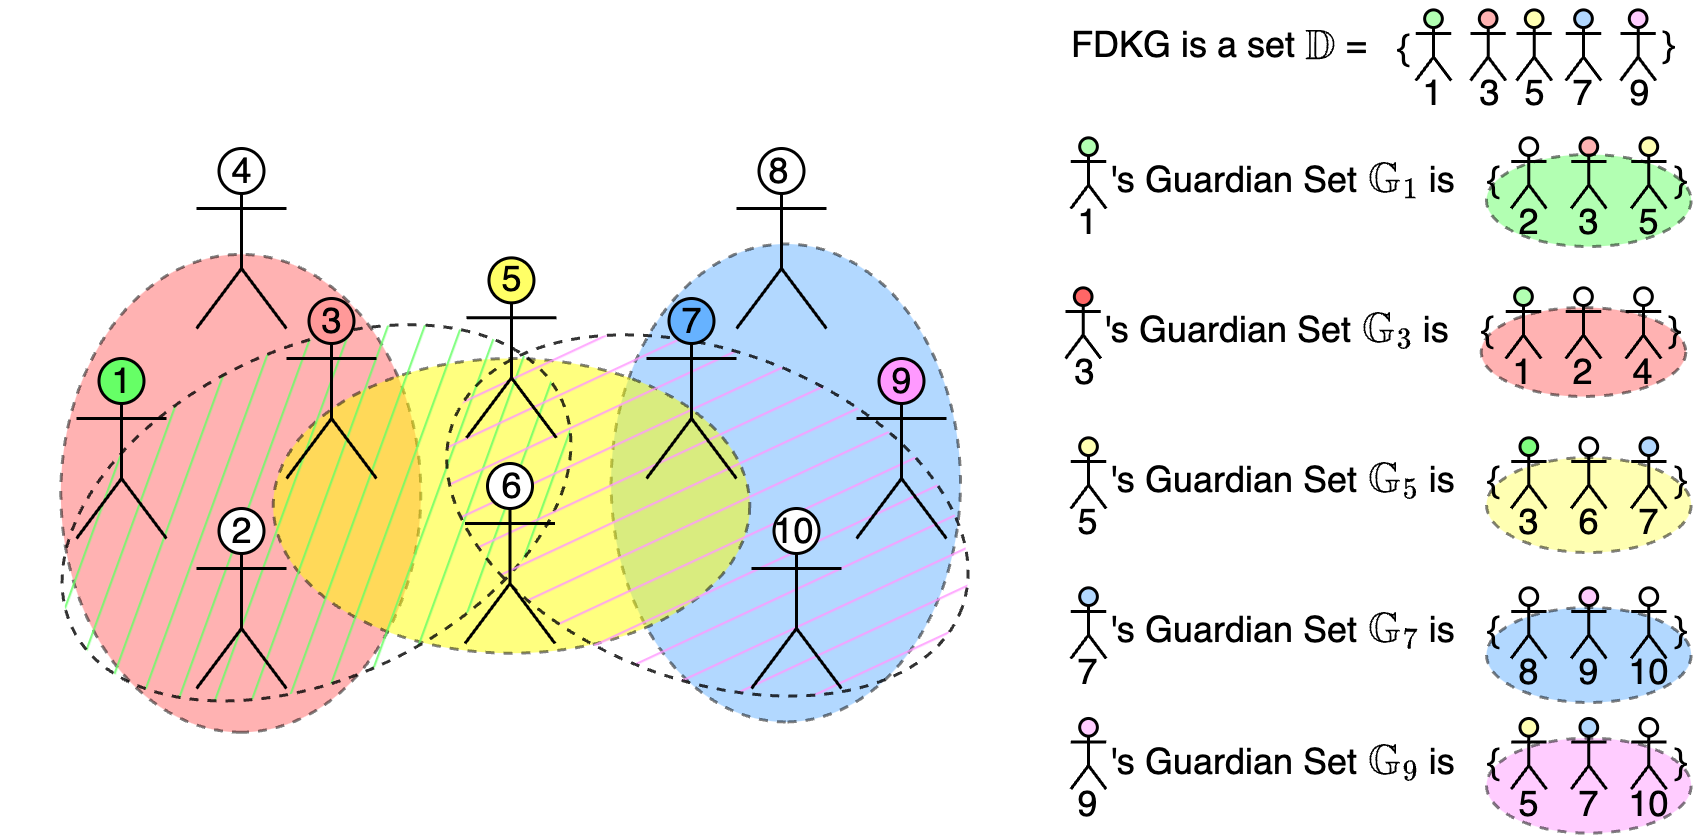
\includegraphics[width=.75\textwidth]{FDKG.png}
    \caption{Example of Federated Distributed Key Generation}
    \label{fig:FDKG}
\end{figure*}

The FDKG process for each participant is as follows:

\begin{enumerate}
    \item \textbf{Party $P_1$}:
        \begin{itemize}
            \item Chooses Guardian Set $\mathbb{G}_1 = \{P_2, P_3, P_5\}$.
            \item Samples a random polynomial $f_1(X) \in_R \mathbb{Z}_q[X]$, computes decryption key $d_1 = f_1(0)$.
            \item Distributes $d_1$ among $\mathbb{G}_1$, yielding shares $\PartialDecryptionKeyShare{1}{2}, \PartialDecryptionKeyShare{1}{3}, \PartialDecryptionKeyShare{1}{5}$.
        \end{itemize}

    \item \textbf{Party $P_3$}:
        \begin{itemize}
            \item Chooses $\mathbb{G}_3 = \{P_1, P_2, P_4\}$.
            \item Samples $f_3(X)$, computes $d_3$, and distributes it among $\mathbb{G}_3$, yielding shares $\PartialDecryptionKeyShare{3}{1}, \PartialDecryptionKeyShare{3}{2}, \PartialDecryptionKeyShare{3}{4}$.
        \end{itemize}

    \item \textbf{Party $P_5$}:
        \begin{itemize}
            \item Chooses $\mathbb{G}_5 = \{P_3, P_6, P_7\}$.
            \item Samples $f_5(X)$, computes $d_5$, and distributes it among $\mathbb{G}_5$, yielding shares $\PartialDecryptionKeyShare{5}{3}, \PartialDecryptionKeyShare{5}{6}, \PartialDecryptionKeyShare{5}{7}$.
        \end{itemize}

    \item \textbf{Party $P_7$}:
        \begin{itemize}
            \item Chooses $\mathbb{G}_7 = \{P_8, P_9, P_{10}\}$.
            \item Samples $f_7(X)$, computes $d_7$, and distributes it among $\mathbb{G}_7$, yielding shares $\PartialDecryptionKeyShare{7}{8}, \PartialDecryptionKeyShare{7}{9}, \PartialDecryptionKeyShare{7}{10}$.
        \end{itemize}

    \item \textbf{Party $P_9$}:
        \begin{itemize}
            \item Chooses $\mathbb{G}_9 = \{P_5, P_7, P_{10}\}$.
            \item Samples $f_9(X)$, computes $d_9$, and distributes it among $\mathbb{G}_9$, yielding shares $\PartialDecryptionKeyShare{9}{5}, \PartialDecryptionKeyShare{9}{7}, \PartialDecryptionKeyShare{9}{10}$.
        \end{itemize}
\end{enumerate}

In a traditional DKG protocol, the minimum set of parties required to achieve Decipherability would be \(\{P_1, P_3, P_5, P_7, P_9 \}\). However, with the FDKG approach and the use of Guardian Sets, this minimum set is reduced to \(M = \{P_3, P_5, P_6\}\), demonstrating the protocol's efficiency in reducing the number of participants required for successful decryption.

\paragraph{Decipherability}
The set $M$ ensures Decipherability because the shares $\PartialDecryptionKey{3},\PartialDecryptionKey{5},\PartialDecryptionKey{6}$ are published directly by these parties, while \PartialDecryptionKey{1} is recoverable by shares \(\{P_3, P_5\}\) and \PartialDecryptionKey{9} is recoverable by shares \(\{P_5, P_7\}\).

\paragraph{Privacy}
Privacy in the FDKG system is compromised when all parties from any Decipherability set collude. In this example, if all parties \(\{P_3, P_5, P_6\}\) collude, they can collectively reconstruct the secret \DecryptionKey{} and therefore decrypt each individual ballot \Ballot{i}.



\section{Experimental Results}

This section evaluates the PeerVote protocol, focusing on proof times and message sizes for two prominent proof systems: Plonk and Groth16, as implemented in the \texttt{snarkjs} WebAssembly (WASM) framework. The execution time for solving the Discrete Logarithm Problem (DLP) in the Offline Tally phase was also evaluated. These experiments were performed on a MacBook Pro with an Apple M1 Pro processor and 16GB of RAM.

\paragraph{Proving Time}

Table~\ref{table:proving-time} shows the time taken to generate a zkSNARK proof for each message using Groth16 and Plonk. The results show a significant performance difference between the two, with Groth16 showing superior efficiency. In particular, during the FDKG phase, Groth16 required a maximum of 2.414 seconds for a 3 out of 4 configuration, compared to Plonk's 146.026 seconds for the same setup.


\begin{table*}
    \centering
    \begin{tabular}{|c|c|c|c|c|c|c|}
    \hline
        \multirow{2}{*}{\textbf{\shortstack{Proving\\ System}}} & \multicolumn{3}{|c|}{\textbf{FDKG}}  & \multirow{2}{*}{\textbf{\shortstack{Encrypt\\ Ballot}}} & \multirow{2}{*}{\textbf{\shortstack{Partial\\ Decryption}}} & \multirow{2}{*}{\textbf{\shortstack{Partial Decryption\\ Share}}} \\ 
        \cline{2-4}
        & \textbf{1 of 2} & \textbf{2 of 3} & \textbf{3 of 4} & &  &  \\ 
        \hline
        \textbf{Groth16} & 1.388 s & 2.135 s & 2.414 s & 0.747 s & 0.619 s & 0.580 s/share \\ 
        \hline
        \textbf{Plonk} & 67.753 s & 71.902 s & 146.026 s & 16.822 s & 16.543 s & 8.137 s/share \\ 
        \hline
    \end{tabular}
    \caption{Proving Time}
    \label{table:proving-time}
\end{table*}

\paragraph{Message Size}

Table~\ref{table:message-size} details the message sizes required in each round of the protocol. Messages using Groth16 are smaller due to their proofs comprising only 3 elliptic-curve points, whereas Plonk-based proofs require 9 points and 6 scalars \cite{gabizonPLONKPermutationsLagrangebases2019}.

\begin{table*}
    \centering
    \begin{tabular}{|c|c|c|c|c|c|c|}
    \hline
        \multirow{2}{*}{\textbf{\shortstack{Proving\\ System}}} & \multicolumn{3}{|c|}{\textbf{FDKG}}  & \multirow{2}{*}{ \textbf{\shortstack{Encrypt\\ Ballot}}} & \multirow{2}{*}{\textbf{\shortstack{Partial\\ Decryption}}} & \multirow{2}{*}{\textbf{\shortstack{Partial Decryption\\ Share}}} \\ 
        \cline{2-4}
        & \textbf{1 of 2} & \textbf{2 of 3} & \textbf{3 of 4} & &  &  \\ 
        \hline
        \textbf{Groth16} & 1152 B & 1568 B & 1984 B & 512 B & 576 B & 768 B/share \\ \hline
        \textbf{Plonk} & 1472 B & 1888 B & 2304 B & 832 B & 896 B & 1088 B/share \\ \hline
    \end{tabular}
    \caption{Sizes of the Messages in Each Round}
    \label{table:message-size}
\end{table*}

\paragraph{Discrete Logarithm Problem (DLP)}

A critical part of the Offline Tally in our protocol involves solving the DLP to extract the number of votes for each candidate. Although typically infeasible, the DLP can be solved by exhaustive search for a small number of voters. Using the method described in \cite{haoAnonymousVotingTworound2010}, we extracted each $x_i$ from the final output point $M$. 

Figure~\ref{fig:dlog-search} shows that solving the DLP follows a power law relationship \( Y = aX^b \), where \( b \) varies linearly with the number of options. This finding suggests that while the time to solve the DLP is linear in the number of voters, it grows exponentially with the number of candidates, posing scalability challenges in larger elections.

\begin{figure*}
    \centering
    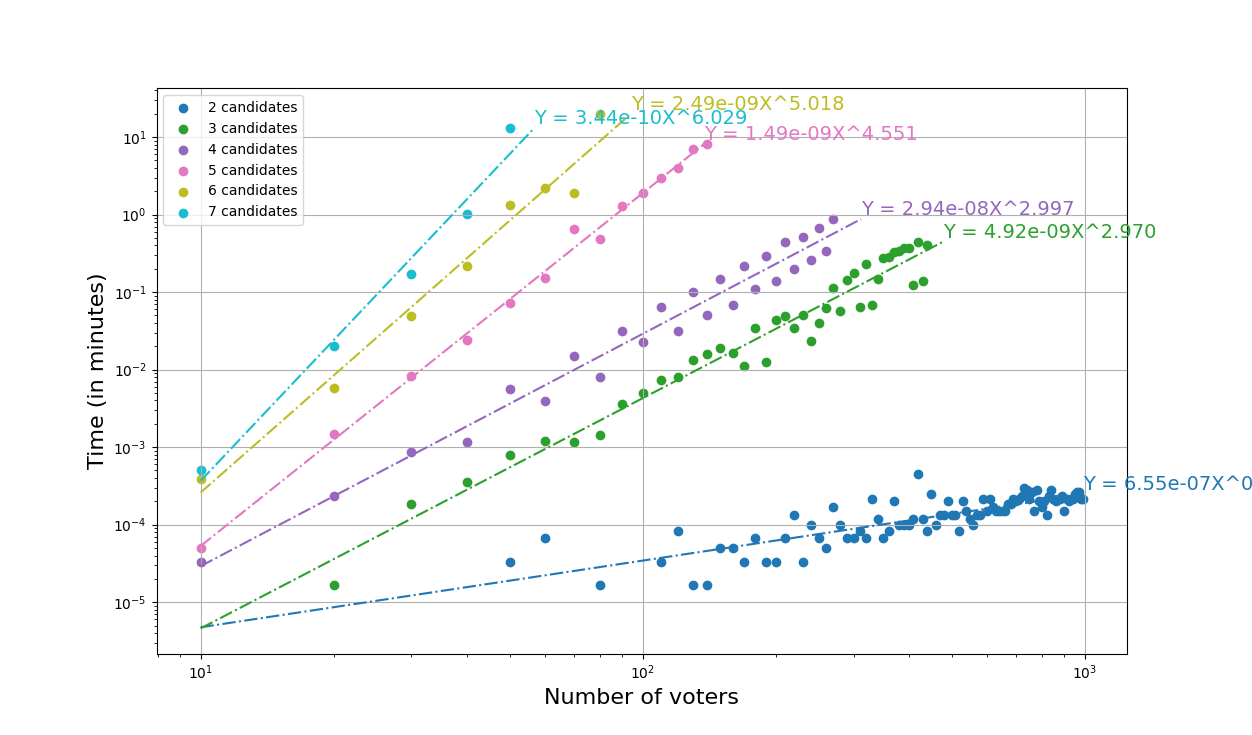
\includegraphics[width=.9\textwidth]{dlog-search.png}
    \caption{Time required to solve DLP with respect to the number of candidates and number of voters (log-log scale).}
    \label{fig:dlog-search}
\end{figure*}

\section{Deployments}\label{sec:deployments}
The protocol can be deployed on any platform that supports message board functionality, i.e. it provides a shared communication space where everyone can post messages and read them all in the same order.
The ideal concept of a message board is difficult to achieve in practice due to the unreliable nature of distributed systems, especially in the presence of Byzantine nodes. 
However, there are many approximations.
In particular, blockchain is the most promising, as it provides the highest level of security in a trustless environment. 
Blockchain comes at the cost of high transaction fees that all interacting parties have to bear. This is the price we want to avoid in democratic voting.
In the future, as the standardisation of the ERC-4337~\cite{ERC4337AccountAbstraction} progresses, transaction fees could be centralised under a single paymaster (e.g. the organiser), allowing gasless voting for participants.

A viable option are peer-to-peer networks. 
We find a promising framework for our protocol in the Wesh Network\footnote{Wesh Network, asynchronous mesh network protocol powered by Berty Technologies' non-profit organisation, \url{https://wesh.network/}}, a toolkit based on the libp2p stack for building peer-to-peer applications.
It is designed for use in a mobile environment, focusing on ease of use, resilience and integrity.

Finally, the PeerVote protocol can be deployed on an centralised messenger platform such as Telegram, Signal or WhatsApp, where the message board is the chat room. This approach is less secure than the previous two, as the central server has potential control over the censorship and order of messages. 

It's worth noting that PeerVote deployed on a central instant messaging platform still provides a high level of security and privacy as all messages are encrypted and authenticated, only the censorship property can potentially be exploited by the central server.

See Figure~\ref{fig:stack-bc} for the conceptual stack of the protocol.

\begin{figure}
    \centering
    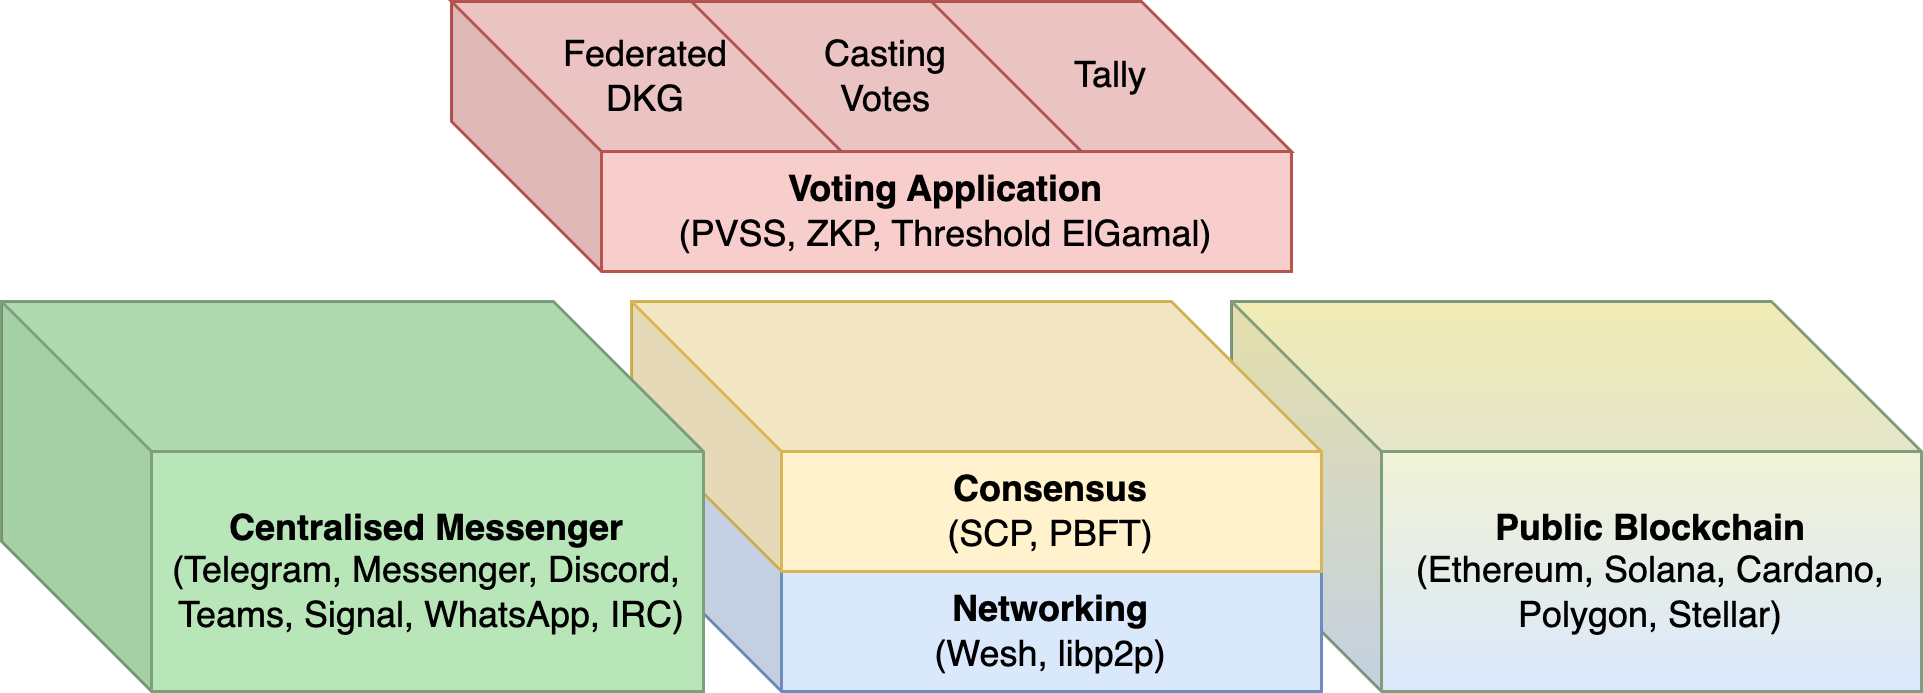
\includegraphics[width=\textwidth]{stack-bc.png}
    \caption{Three possible deployments of the protocol: Centralised messenger, ad-hoc peer-to-peer network, and public blockchain.}
    \label{fig:stack-bc}
\end{figure}

\section{Discussion and conclusion}

Our work introduces a robust voting protocol that eliminates reliance on centralised entities and demonstrates resilience to node unavailability. Federated Distributed Key Generation (FDKG) is our main innovation, extending traditional Distributed Key Generation (DKG) methods. FDKG uniquely allows key reconstruction by parties within their Guardian sets, in addition to those participating in the original DKG. This generalisation of DKG—where standard DKG is equivalent to a 0-of-k FDKG protocol—significantly improves the robustness of the protocol by minimising the size of the decipherability sets while preserving privacy, where these sets include the most trusted parties in the network.

The protocol's robustness is particularly valuable in contexts with uncertain network reliability and participant availability, ensuring secure and uninterrupted voting processes. Future research could include simulating real-world trust dynamics in communities to assess the applicability of the protocol \cite{healdMathematicalDescriptionTrust2019}.

However, implementing zkSNARKs for message attestation involves a trade-off between setup complexity and computational efficiency. Trusted setup ceremonies, such as those used in Groth16 \cite{grothSizePairingbasedNoninteractive2016}, offer greater efficiency compared to transparent setups such as Plonk \cite{gabizonPlonkPermutationsLagrangebases2019a}. Our experiments showed that on a high-end personal computer, Groth16's verification time per message was 1-3 seconds, while Plonk required 16-145 seconds. Although trusted setups involve strong assumptions, they are a one-time requirement and can be reused in future votes, a common practice in zkSNARK-based protocols.

A critical aspect of our protocol is offline tallying, which relies on solving the Discrete Logarithm Problem (DLP). The complexity of this task follows a power law \( Y = aX^b \), where \( X \) is proportional to the number of voters and \( b \) increases with the number of candidates, implying linear growth with the number of voters and exponential growth with the number of candidates. The computational challenge can be partially mitigated by parallelizing the exhaustive search over all parties. The overall time complexity would be reduced to $\frac{1}{n}$ time. Overcoming this scalability challenge remains an area for future improvement, possibly through the development of more efficient algorithms.

Three deployment options for our protocol are proposed (see Figure~\ref{fig:stack-bc}): as a peer-to-peer application using Wesh Network, or as a smart contract on public blockchains using ERC-4337~\cite{ERC4337AccountAbstraction} to centralise voting costs under a single paymaster (e.g., organiser), allowing gasless voting for participants, or via a centralised messenger application such as Telegram, WhatsApp, Signal or Discord.

We have open sourced the implementation of our protocol in TypeScript and Golang to facilitate widespread use and improve accessibility. The codebase is available at \url{https://github.com/anonymised/for/review}

Optimization avenues include improving proof times and sizes by batching proofs or reformulating them into more efficient Sigma Proofs. Another path involves on-chain implementation with gasless transactions, leveraging ERC-4337's paymaster concept.

In the future, the anonymity of the voters could be additionally protected from collusion by the malicious parties by using zero-knowledge set membership proofs~\cite{Semaphorea}, as seen in protocols like Cicada~\cite{BuildingCicadaPrivate} and Vocdoni~\cite{VocdoniIntroductionVocdoni}. In this way, although the colluding parties could decrypt individual ballots, they could not determine who had cast them.

Coercion resistance is another property that could improve the PeerVote protocol. While Daian et al.~\cite{daianOnChainVoteBuying2018} argue that achieving coercion resistance in a permissionless environment without trusted hardware is impossible, various strategies have been explored that come close to the ideal model. These include allowing voters to submit multiple votes, with each new vote overriding the previous one~\cite{VocdoniIntroductionVocdoni}, and allowing signing key changes to invalidate any subsequent votes signed with the old key~\cite{ethereumfoundationMinimalAntiCollusionInfrastructure2022, PrivacyscalingexplorationsMaci2023}. We plan to extend the protocol with both of these mechanisms in the future.

In conclusion, our protocol represents a significant step forward in the evolution of Internet voting systems. By embracing decentralisation, enhancing security and prioritising privacy, we aim to contribute to the development of more resilient, trustworthy and inclusive voting mechanisms in the digital age. As we continue to refine and optimise our protocol, we remain focused on the broader goal of modernising democratic processes and empowering communities with reliable and accessible voting technologies.

% \section*{Acknowledgements}
% We would like to thank Lev Soukhanov for his crucial role in designing the voting protocol and the Delendum team for their support and valuable insights during our research fellowship. We are grateful to Maya Dotan for her detailed review and helpful feedback, which significantly improved the quality and clarity of our work.

\bibliographystyle{splncs04}
\bibliography{bibliography}

\appendix

\section{Private Channel}
\label{private-channel}
Each user uses a private, authenticated channel to send encrypted messages to other parties. We use ElGamal encryption on the BabyJub curve as described in \cite{ElGamalEncryptionDecryption2020,jieWeijiekohElgamalbabyjub2023}. The encryption process starts with a plaintext scalar $m$, which is transformed into a point on the BabyJub elliptic curve by generating a random value $r$, computing the message $M=r\G$ and the x-increment $\Delta$, which must be added to the plaintext to obtain the x-value of $M$. Thus, the ciphertext consists of two elliptic curve points and a field element $(C_1, C_2, \Delta=M.x - m)$. The complete encryption process is described in detail in Algorithm~\ref{alg:encryption}.

Decryption of the ciphertext $(C_1, C_2, \Delta)$ follows the standard ElGamal method, with the addition of $\Delta$ to the x-coordinate of the starting point, as described in Algorithm~\ref{alg:decryption}.

\begin{algorithm}
    \SetAlgoNlRelativeSize{0}
    \SetAlgoNlRelativeSize{-1}
    \SetAlgoNlRelativeSize{1}
    \SetKwInOut{Input}{Input}
    \SetKwInOut{Output}{Output}
    \caption{$\texttt{Enc}_{P_i}$}
    \label{alg:encryption}
    
    \Input{A scalar $m$}
    \Output{A tripe $(C_1, C_2, \Delta)$}
    
    $k \gets_R \mathbb{Z}_q$\;
    $r \gets_R \mathbb{Z}_q$\;
    $C_1 = kG$\;
    $M = rG$\;
    $C_2 = kP + M$\;
    $\Delta = M.x - m$\;
    \Return $(C_1, C_2, \Delta)$
\end{algorithm}

\begin{algorithm}
    \SetAlgoNlRelativeSize{0}
    \SetAlgoNlRelativeSize{-1}
    \SetAlgoNlRelativeSize{1}
    \SetKwInOut{Input}{Input}
    \SetKwInOut{Output}{Output}
    \caption{$\texttt{Dec}_{s_i}$}
    \label{alg:decryption}
    
    \Input{A tripe $(C_1, C_2, \Delta)$}
    \Output{A scalar $m$}
    
    $M = C_2 - s_i C_1$\;
    $m = M.x - \Delta$\;
    \Return $m$
\end{algorithm}
\end{document}
